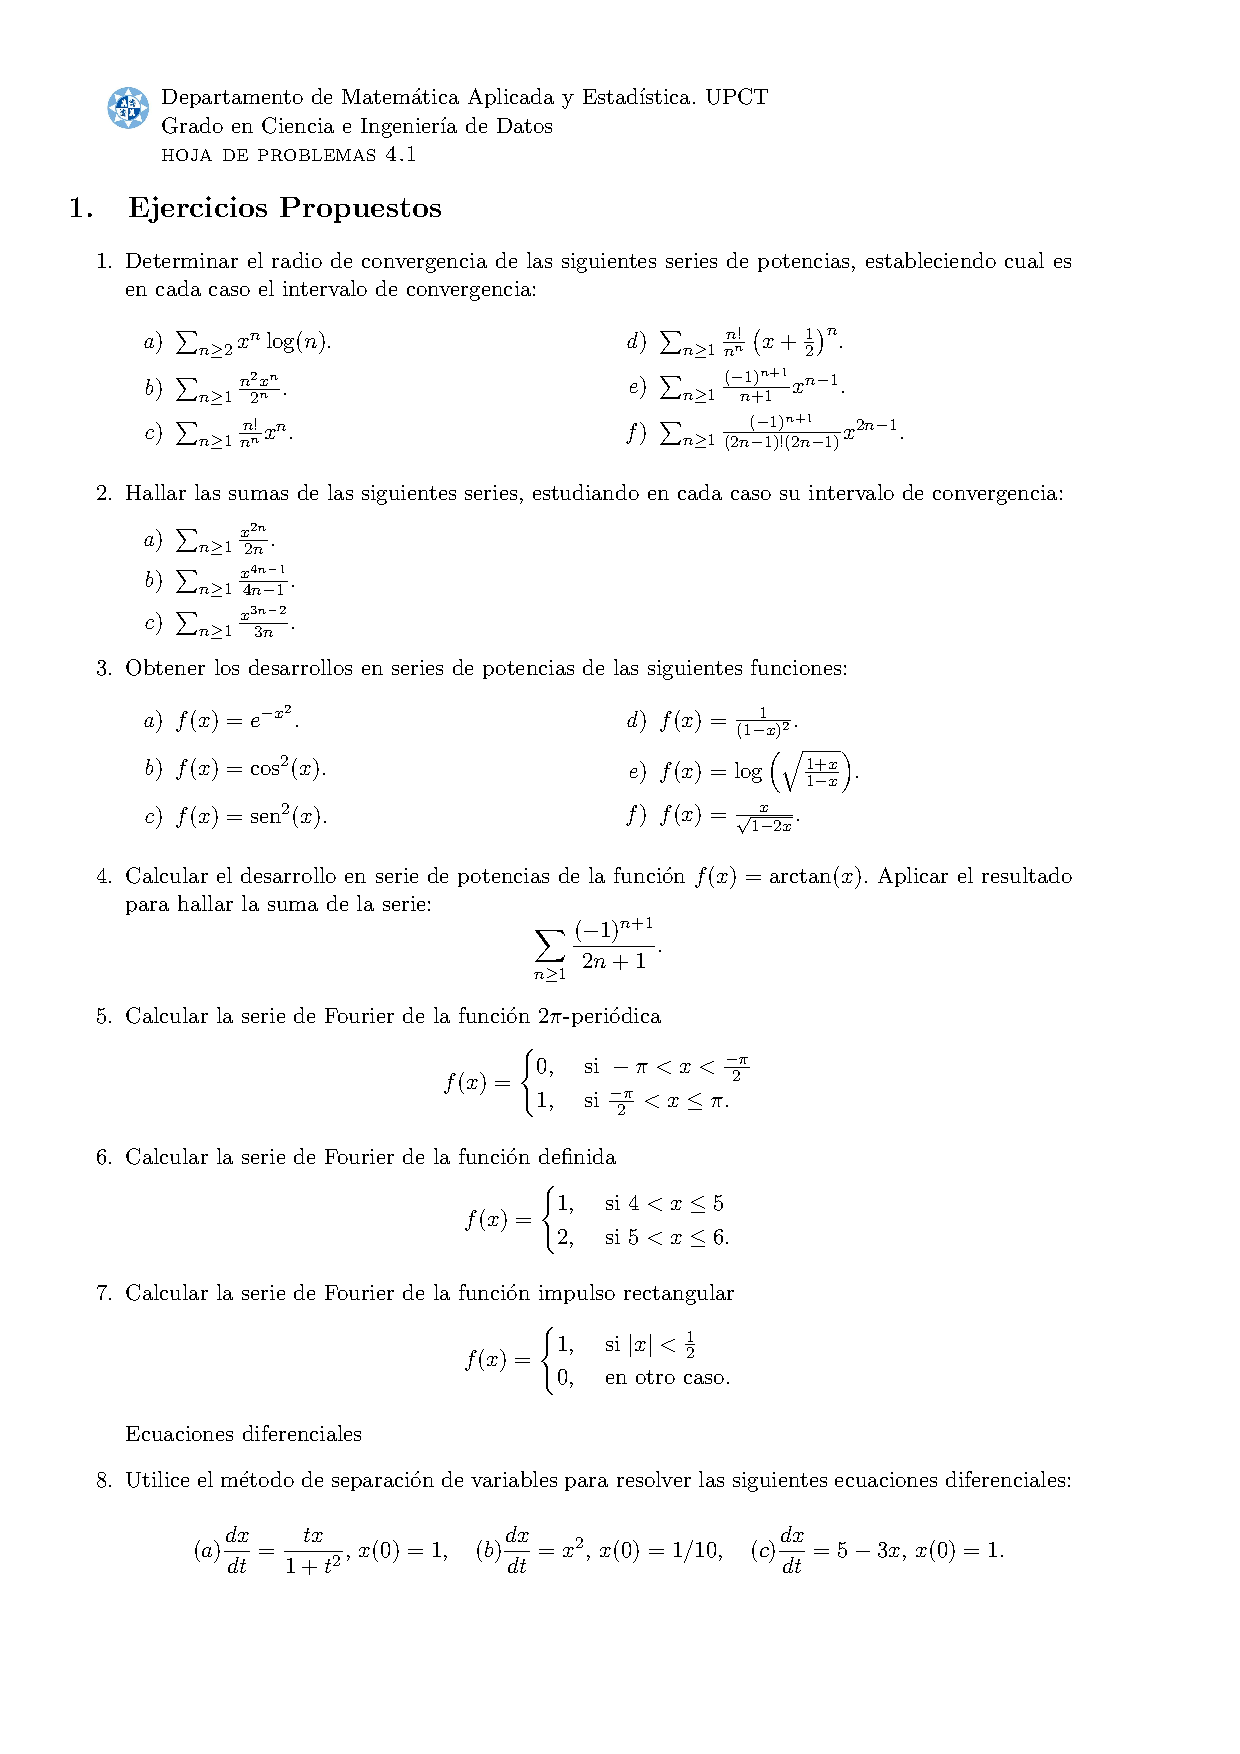
\includepdf[pages=-]{Tareas/Tema 4/Hoja 4.1.pdf}

\begin{enumerate}[label=\color{red}\textbf{\arabic*)}]
      \item \lb{Determinar el readio de convergencia de las siguientes series de potencias, estableciendo cual es en cada caso el intervalo de convergencia.}
      
      \begin{enumerate}[label=\color{red}\alph*)]
            \item $\db{\sum_{n\ge2}x^n\log(n)=}\sum_{n\ge2}a_n\cdot(x-x_0)^n$
            
            $\begin{array}{l}
                  a_n=\log(n)\\
                  x_0=0
            \end{array}\qquad\varphi=\lim_{n\to\infty}\left|\dfrac{a_n}{a_{n+1}}\right|=\lim_{n\to\infty}\left|
            \dfrac{\log(n)}{\log(n+1)}\right|=1$
      \end{enumerate}
\end{enumerate}